%!TEX root = ../thesis.tex
\chapter{Trading strategies based on Hidden Markov Models}

\if
pdf
    \graphicspath{{Chapter5/Figs/Raster/}{Chapter5/Figs/PDF/}{Chapter5/Figs/}}
\else
    \graphicspath{{Chapter5/Figs/Vector/}{Chapter5/Figs/}}
\fi

\section{Selected Market Emissions}

	There is a huge number of observable variables that one could abstract from cryptocurrency market. A possibility of discrete states within the given state space is plausible and feasible, it would, given our model constraints, provide poor inference since additional information would remain hidden. Imagine a situation where our observable states are defined as a relative change in price or a sudden drop/uprise in the traded volume on the exchange. In order to discreticize our states and construct transition and emission probabilities we are forced to construct intervals that would well represent the boundaries upon which the model defines structure and predictions. 
	
Assuming that the price increase in   the idea predefined Hidden Markov Model will assume
	
	However it is much more efficient to assume continuity in our predefined observable states. It is nowadays empirically proved, as in (citace) that using technical indicators as predictors for the future spot price yields more accurate machine learning models. As will be demonstrated each of the technical indicators can be classified into several families of indicators, such as momentum, volume, volatility and cycle indicators. For our purposes we will consider mainly momentum indicators that are calculated using Open, High, Low, Close prices (hereinafter "OHLC") and Volume indicators. There is a huge variety of technical indicators to choose from therefore the selection was made according the most used and well known indicators or their transformed versions. 

In our case we will consider following observable states that will be defined and elaborated on in the upcoming sections:

\begin{itemize}
\item[1)] Moving Average Convergence/Divergence (MACD)
\item[2)] Stochastic Oscillator
\item[3)] Chaikin Oscillator 
\item[4)] Relative Strength Index (RSI)
\item[5)] Aroon Oscillator 
\end{itemize}


\subsection{Moving Average Convergence Divergence}

Also knows as MACD is a trend-following momentum indicator that represents the differences between two exponential moving averages (hereinafter "EMA"). The most common and traditional moving averages are 26-period EMA and 12-period EMA. 

The indicator is often used with so-called ""signal line" that is constructed as a 9-period EMA and is used as a trigger for a buy and sell signal. In practical application a trader decides to buy a stock if the signal line crosses MACD line from above and sell if it crosses from below, assuming simplistic trading strategy using only MACD. EMA also called exponentially weighted moving average is a type of moving average that differs from weighted moving average WMA by the distribution of weights to past observations. While WMA considers the linearly decreasing distribution of weights, the EMA assumes exponential decrease in weights. Furthermore it is necessary to elaborate over the values of weights because it might not always be unambiguous. WMA distributes weights chronologically and linearly, e.g. 10-period WMA gives weight 1 to the earliest observation and 10 to the most recent observation, the case within EMA is often not that simple. The weights given to each observation are computed as $(1 - \lambda)^i$ where $i \in \mathbb{N}_0$ and is bounded from above by the assumed period of interest, e.g. 3, 10, 26-period denoted as T for the sake of . As $i$ increases identically with the time lag the value of weights decreases. The important role that ought to be questioned is the parameter $\lambda$ that is defined as $\frac{k}{T+1}$ where k represents the so called "smoothing" parameter. Traders and analysts use value 2 for the smoothing parameter but the number may be defined on the interval $(0,T)$. Higher values of k mean bigger weights given to most recent observations. 

The Figure 2.1 illustrates MACD line, signal line as well as "MACD histogram" which is displayed as a bar chart indicating the difference of the former ones. Traders use such a distance to identify whether the bullish or bearish momentum is high, i.e. bigger the distances of these two lines higher the price momentum.

MACD has its unfortunate limitations that mainly arise from the non-trending moments. When the price enters sideways movement the MACD histogram signals decreases distances between MACD and signal line, the trend reversal is possible but the price moves sideways which eventually results in false positive signal. Moreover when the price moves sideways for longer periods MACD may signal too many false trend reversals. The most common practice for traders is to combine MACD signals with other indicators such as Relative Strength index (RSI) that measures overbought or oversold market. The RSI uses average price gains and losses usually over 14 periods and yields values between 0 and 100, indicating overbought market for values 70 (80) to 100 and 30 (20) to 0 for oversold market. The idea is that when the distances between MACD line and signal line increase and RSI signals overbought market the trader might consider this as a strong trend reversal signal. The idea is that signals from MACD strategy often produce false signals when price suddenly moves sideways and RSI helps to indicate the false positive signal. 

\begin{figure}[ht]

\begin{center}
	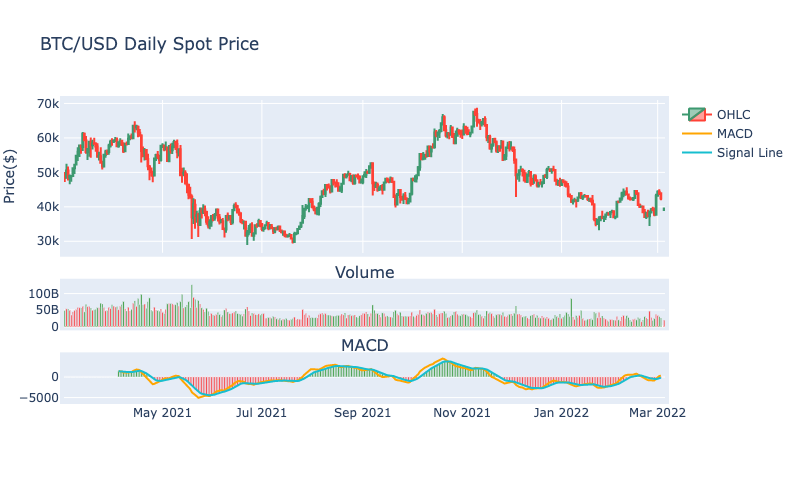
\includegraphics[width=0.9\textwidth]{Figs/MACD.png}
\end{center}

\caption{\textit{ Candlestick graph of daily spot price of BTC/USD from March 2021 to March 2022 with subplot containing two lines for MACD and Signal line and a bar chart as their difference}}

\end{figure}

\subsection{Stochastic Oscillator}

	A Stochastic Oscillator is a momentum indicator that compares the most recent closing price of a security with its predeceasing ones. Naturally, the range of preceding closing prices or the range of closing prices is 14 periods but it is regular that such an assumption is often edited to best fit the current needs of a trader. Also slight variation in taking the (weighted) moving average of the oscillator values is often introduced. The indicator is used to generate trading signals that refer to the current overbought state of the market, which means that the indictor values range from 0 to 100 where the values closer to the number 0 indicate oversold market and inversely values closer to 100 overbought market. 
	
Stochastic Oscillator is computed as follows:

\begin{equation}
SO_{t} = \frac{C_{t-1} - L_{14}}{H_{14} - L_{14}}
\end{equation}

where $C_{t-1}$ denotes the most recent closing price of a security, $H_{14}$ and $L_{14}$ are the highest and lowest price traded during 14-period interval respectively. $SO_{t}$ is sometimes referred to as a "fast" stochastic indicator. As said before this interval may be changed arbitrarily. Traders also developed so called "slow" Stochastic Oscillator which is defined as a 3-period moving average of $SO_{t}$. Thus when Stochastic Oscillator crosses the smooth "Slow" Stochastic Oscillator a trading signal is generated.

Considering values above 80, the indicator signals overbought market and oversold market when the value drops below 20. Although it remains to hold true that the indicator often produces false indications that may be caused by periods of time where the price remains overbought/oversold for some time and trading with respect to such oscillator may result in losses. It is rather recommended to observe the values of stochastic oscillator and use it for trend reversal indication. 

\begin{figure}[ht]

\begin{center}
	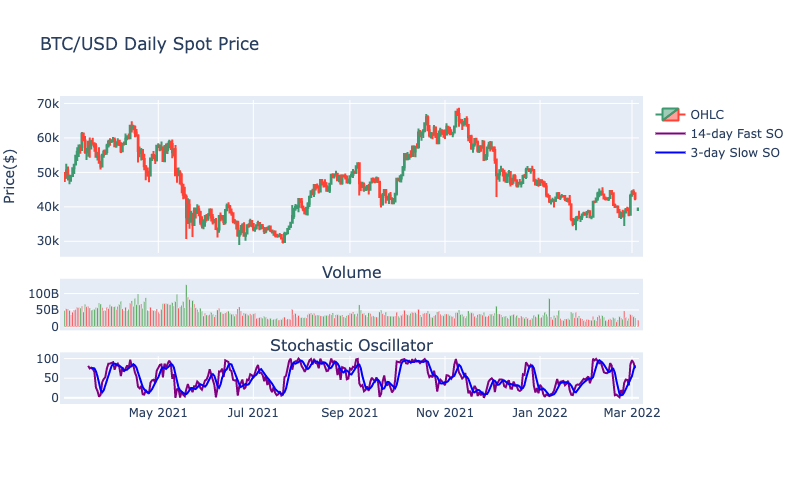
\includegraphics[width=0.9\textwidth]{Figs/Stochastic.png}
\end{center}

\caption{\textit{ Candlestick graph of daily spot price of BTC/USD from March 2021 to March 2022 with subplot with line indicating Stochastic Oscillator}}

\end{figure}

\newpage

\subsection{Chaikin Oscillator}

Chaikin Oscillator is a momentum based indicator of the Accumulation/Distribution Line (hereinafter "A/D line"), which is a cumulative indicator that aims to identify potential divergences between stock price and trading volume. The oscillator is calculated as a difference between 3- day and 10-day Exponential Moving Average of A/D line. 

\vspace{0.5cm}

The calculation of the Chaikin Oscillator may be broken down into several steps:
\begin{itemize}
\item[(i)] First, we ought to calculate the Money Flow Multiplier for each time step denoted by "N".

\begin{equation}
N_{t} = \frac{(Close_{t} - Low_{t}) - (High_{t} - Close_{t})}{High_{t} - Low_{t}}
\end{equation}

\item[(ii)] Now we may multiply $N_t$ by the trading volume in given period of time to get the Money Flow Volume denoted as $M_t$. With that we recursively construct the A/D line as:

\begin{equation}
ADL_t = M_{t-1} + M_t
\end{equation}

\item[(iii)] Given the constructed A/D line, we compute the Chaikin Oscillator values as a difference of 3-day and 10-day exponential moving averages.

\begin{equation}
CO_t = \frac{\sum_{i=0}^{3} {(1-\alpha)}^i*Close_{t-i}}{\sum_{i=0}^{3} {(1-\alpha)}^i} - \frac{\sum_{i=0}^{10} {(1-\beta)}^i*Close_{t-i}}{\sum_{i=0}^{10} {(1-\beta)}^i}
\end{equation}

where we assume that the weights denoted as $\alpha$ and $\beta$ are computed as $2/(days + 1)$. Numerator as a smoothing factor is often declared as 2. However, the indicator may be set to absolutely different number between 0 and 1 according to the needs and assumptions made by the trader/analyst, therefore setting the parameter close to 1 is putting more weight to the most recent price.

One way to interpret the indicator is to trade with respect to the time when the Chaikin Oscillator crosses zero from below and above which signals buy and sell signals respectively.

\end{itemize}


\begin{figure}[ht]

\begin{center}
	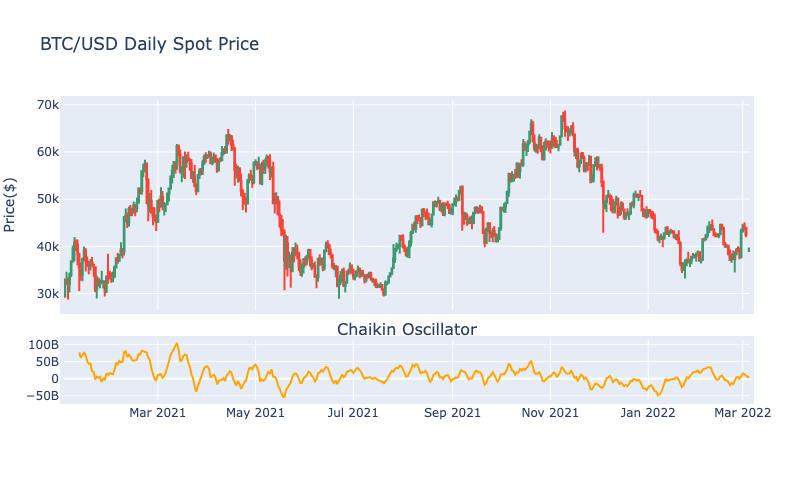
\includegraphics[width=0.9\textwidth]{Figs/Chaikin.png}
\end{center}

\caption{\textit{ Candlestick graph of daily spot price of BTC/USD from March 2021 to March 2022 with subplot indicating Chaikin Oscillator}}

\end{figure}


\subsection{Relative Strength Index}

Given the recent price changes Relative Strength Index measures its magnitude in order to indicate the overbought or oversold market. In technical analysis such indicator is represented by an oscillator ranging from values 0 to 100. Empirically 
it was determined that values above 70 and below 30 signal overbought and oversold asset respectively. Therefore, we may also use RSI to produce buy and sell signals from former logic, which means that when the RSI crosses 30 from below, buy signal is generated as well as sell signal in case it crosses 70 from above. We also could measure the strength and continuation of the trend for cases in which the RSI crosses value of 50. Such interpretation results from the RSI formula where the value of 50 means that the average gain equals the average loss in the last period.

The formula below explains the procedure within which the values of RSI are calculated. It is obvious that the RSI rises as the number of positive closing prices increases, i.e. the relative change in prices is positive, and falls if otherwise. The standard time interval for  the calculation is 14 preceding periods with respect to $t$, hereby denoted as $T$.

\begin{equation}
RSI_t = 100- \frac{100}{1+r_t} 
\end{equation}
 
 where r is a ratio of average gains and losses as follows:
 
\begin{equation}
 r_t = \abs{\frac{\sum_{i=1}^{T}(\frac{P_{t-i+1}}{P_{t-i}}-1)\mathbbm{1}_{[P_{t-i+1} - P_{t-i} > 0]}}{\sum_{i=1}^{T}(\frac{P_{t-i+1}}{P_{t-i}}-1) \mathbbm{1}_{[P_{t-i+1} - P_{t-i} < 0]}}}
\end{equation}

given that $P_t$ denotes the value of an asset at time $t$.

As stated before there are several drawbacks of using the RSI as a trading indicators only by itself, it happens that the price usually rises and stays overbought for a substantial period of time in times of significant and strong bullish trend. RSI as an oscillator is used as an auxiliary trading tool below the price chart:

\begin{figure}[ht]

\begin{center}
	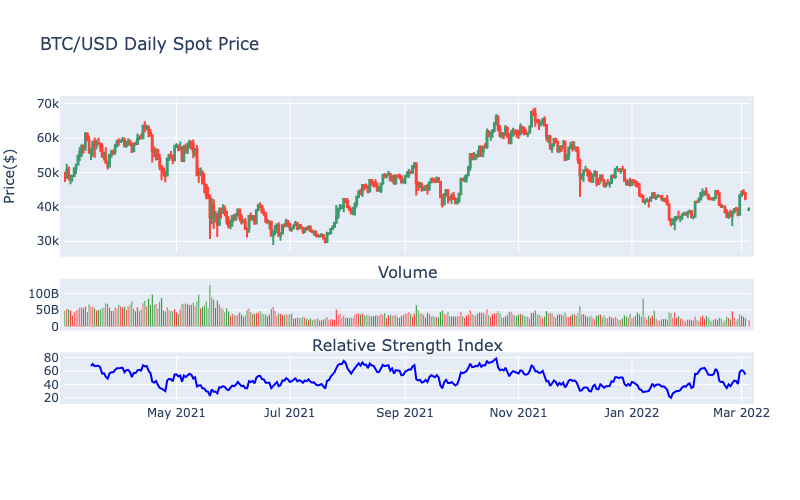
\includegraphics[width=0.9\textwidth]{Figs/RSI.png}
\end{center}

\caption{\textit{ Candlestick graph of daily spot price of BTC/USD from March 2021 to March 2022 with a subplot containing  RSI}}

\end{figure}

\subsection{Aroon Indicator}

Aroon indicator is used for trend reversal identification and a measure of its strength. Indicator is composed out of two lines aroon up and aroon down that measure the time between new highs or lows respectively. Alternatively, they measure the strength of a bullish or bearish trend. Obviously the main idea of the indicator is based upon the fact that bullish trends are naturelly formed by subsequently creating new highs while bearish trends form new lows. Aroon Up and Aroon Down are computed as follows:

\begin{equation}
Aroon Up = \frac{25 - h}{25} * 100
\end{equation}
 
\begin{equation}
Aroon Down = \frac{25 - l}{25} * 100
\end{equation}

Where $h$ represents the number of periods from the last 25-period High and $l$ the number of periods from last 25-period Low. 

The interpretation of the indicator is very intuitive since the situation in which the Aroon Up line is above Aroon Down line signals bullish trend and when these two lines cross the signal of the trend reversal is generated. That also implies that for higher values of Aroon Up the bigger the strength and for lower values the uptrend is weaker and vice versa. In practice the crossover of these two lines is what generates the buy or sell signals, i.e.\ if Aroon Up crosses Aroon Down line from below a buy signal is generated and vice versa. 

Although, Figure 2.4 graphically illustrates the Aroon Up and Down lines well, it is simpler to transform these two lines into one oscillator that would produce buy or sell signal in the case of zero crossover from above and from below. That is achieved by subtracting Aroon Up and Aroon Down line creating Aroon Oscillator.

\begin{figure}[ht]
\begin{center}
	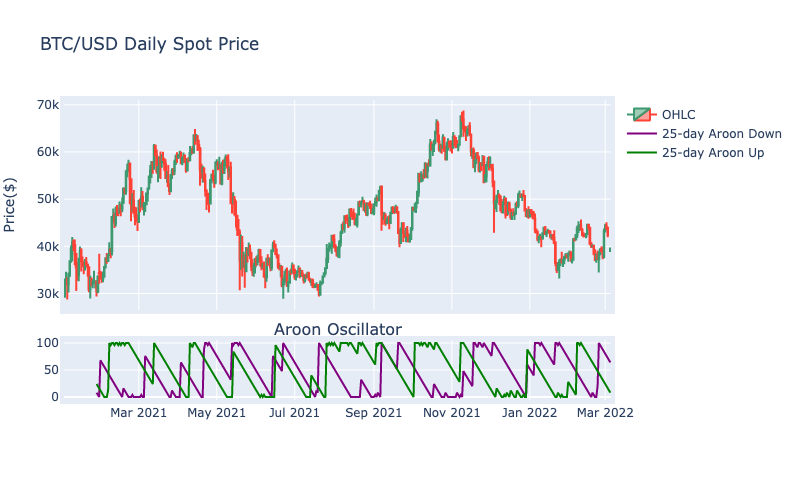
\includegraphics[width=0.9\textwidth]{Figs/Aroon.png}
\end{center}
\caption{\textit{Candlestick graph of daily spot price of BTC/USD from March 2021 to March 2022 with subplots containing two lines for Aroon Up/Down Indicator and Aroon Oscillator}}
\end{figure}

\section{Market regimes and trading strategies}

\subsection{Market states}

\subsection{Trading strategies}